% Chapter Template

\chapter{Nucleosynthesis} \label{ch:nucleo}% Main chapter title

%% =======================================================
%%
%%                   Nucleosynthesis
%%
%% =======================================================

%\textcolor{red}{Based on the Jones Lippuner PhD thesis}

%For a long time the general consensus was that all elements in the universe 
%were synthesized during the Big Bang \citep{Alpher:1948}. Later studies have, however, 
%proven that only elements with atomic number $A<8$ were produced 
%(see \eg, \citet{Alpher:1950,Shaviv:2012}). Thus, only the lightest elements, hydrogen 
%and helium primarily, were produced during in the Big Band \citep{Burbidge:1957}. 
%Heavier elements are synthesized in a plethora of processes that we briefly recall here.

%In this chapter we discuss \nuc{} that occurs in the matter ejected in \ac{BNS}
%mergers, focusing on the rapid neutron capture process (\rproc{}) responsible 
%for the creation of heavy elements \citep{Burbidge:1957}. 
%
In Sec.~\ref{sec:intro:nucleo} we introduced conditions for and cites of
\rproc{} \nuc{}, and its contribution to the Universe' chemical evolution. 
Here, we briefly discuss how numerous nuclear species, participating in thousands on nuclear 
reactions, are evolved using the novel \texttt{SkyNet} nuclear reaction network code, and how the process can be paramtrized for quick 
calculations of final abundances in \ac{BNS} merger ejecta.
%
Then, we consider \ac{BNS} mergers as a source of \rproc{} elements. 
We compute the nucleosynthetic yields from merger simulations 
discussed in the chapter~\ref{ch:bns_sims}.

%\red{
%[Lippuner 221 page] Note that luminosity of the electron anti-neutrino is higher then the one of the 
%electron neutrino due to \magenta{re-leptonization} of the neutrino emitting disk \cite{Foucart:2015gaa}.
%}

%\section{Heaviest elements in the Universe}
%\label{sec:nuc:rproc}




%% =======================================================
%%
%%                   Nucleosynthesis SkyNET
%%
%% =======================================================

\section{Modeling the nucleosynthesis}

Nuclear reactions play an important role in numerous astrophysical cites, where sufficiently high temperatures 
and densities are achieved. 
%In particular, in main sequence stars nuclear fusion prevents stars from collapsing, releasing the binding energy, 
%counteracting gravity \citep{Bethe:1939}. When stars do undergo a core collapse, the nuclear and weak reactions 
%govern the explosion by introducing and removing energy (\eg, via neutrino cooling and heating). 
%%
%A small amount of the material synthesized in the explosive burning is ejected into the \ac{ISM}  
%\citep{Nomoto:1997if,Woosley:2002}. It is composed mostly of iron-group elements, enriched with heavier elements 
%synthesized in weak \rproc{} \citep{Wanajo:2013} and \sproc{} \citep{Burbidge:1957}. 
%Enrichment of \ac{ISM} with even heavier elements, synthesized in full \rproc{}, is believed to occur manly in 
%compact binary mergers \citep{Freiburghaus:1999}, \red{where the material with ifferent composition is ejected on 
%    a prolonged timescale via numerous physical processes [ManyRefs]}.
% \gray{In addition, nuclear burning in a form of thermonuclear explosion occurs when matter is accreted onto a 
%     white dwarf or a neutron star, producing electromagnetic transients Novae and X-ray bursts \cite{Boyd:2008,Freiburghaus:1999}}
%
%% ========== INTORCUTION TO NRN 
To study the \nuc{} in different physical environments, it is necessary to model nuclear reactions focusing 
not only on the total energy generation \citep[\eg][]{Weaver:1978,Mueller:1986,Timmes:1999} but tracking the 
evolution of the whole ensemble of nuclear species. A mathematical and/or numerical model that describes 
coupled nuclear reactions, tracking the evolution of abundances of various species, coupled by a non-linear 
reaction, rates is called \ac{NRN}.
%
% BBN
The complexity of a network, \ie, the number of species and reactions evolved 
varies depending on the intended implementation. 
%
%For instance, for a \ac{BBN} rarely more then a dozen nuclear species are evolved 
%\citep{Wagoner:1973,Orlov:2000,Nollett:2000fh,Coc:2013eha,Cyburt:2015mya}. 
%
%% STellar
%Stellar evolution models also included reaction networks starting from a few species and reactions 
%\citep[\eg][]{Hayashi:1962,Hofmeister:1964} and incorporating tens or even hundreds of them in a more 
%recent and advanced models \citep{Arnett:1977,Weaver:1978,Paxton:2011,Bressan:2012,Jones:2015}
%
%% SN
%Networks designed for explosive nuclear burning and supernovae evolved from including a few tens of species 
%\citep[\eg][]{Truran:1966,Truran:1967,Arnett:1969,Woosley:1973} to including hundreds of species and reactions, 
%(\eg, in type Ia \acp{SN} \citep{Thielemann:1986,Hillebrandt:2013gna,Seitenzahl:2013,Leung:2015fxa}, in \acp{CCSN} 
%\citep{Thielemann:1986,Limongi:2003ui,Heger:2008td,Harris:2014}, in novae 
%\citep{Weiss:1990,Jose:1997vf,Iliadis:2002zz,Starrfield:2016} and X-ray bursts 
%\citep{Schatz:2001xx,Woosley:2003cd,Cyburt:2010,Parikh:2012hx}) 
%
% r-process 
For instance, neutron capture results in a creation of unstable nuclides, 
that decay via complex chains of reaction, involving hundreds and thousands of steps. 
Thus, \acp{NRN} have to be adequately complex for modeling 
the \sproc{}, \citep[\eg][]{Prantzos:1990,Kaeppeler:2011,Nishimura:2017zdi} 
and even more so to model \rproc{}. 
%
Targets for such studies include 
\acp{CCSN} neutrino driven winds \citep[\eg][]{Woosley:1992,Arcones:2010,Wanajo:2013},
and outflows from magnetorotational \acp{CCSN} \citep[\eg][]{Winteler:2012,Nishimura:2015nca}.
In compact object mergers several cites with different conditions 
require modeling (See Sec.~\ref{sec:intro:merg_pmerg} and % that include ejecta,
%\citep{Goriely:2011vg,Bauswein:2013yna,Wanajo:2014wha,Just:2014fka,Fernandez:2016sbf}\red{[Refs]}, 
%and a disk (torus) formed after merger around the remnant 
%\citep{Surman:2008qf,Perego:2014fma,Martin:2015hxa,Lippuner:2017tyn}.
%
%This however does not limit the scope of where modeling of neutron capture nucleosynthesis is done. 
\citet[\eg][]{Blinnikov:1996,Panov:1995,Panov:2001,Mumpower:2011ar,Lippuner:2018phd} for an overview.

% Other NRN codes
Several nuclear reaction networks are available in the literature. 
In particular: a set of networks by 
\citet{Timmes:1999}\footnote{\url{http://cococubed.asu.edu/code_pages/burn.shtml}}, 
\texttt{XNet} by \citet{Hix:1999}\footnote{\url{http://eagle.phys.utk.edu/xnet/trac}} , 
\texttt{NucNet} by \citet{Meyer:2007}\footnote{\url{https://sourceforge.net/projects/nucnet-tools}}
and \texttt{SkyNet} by \citet{Lippuner:2015gwa}\footnote{\url{https://bitbucket.org/jlippuner/skynet}}.
%
The latter is a popular choice studying nucleosynthesis in neutron rich environment
\citep{Lippuner:2015gwa,Radice:2016dwd,Roberts:2016igt,Lippuner:2017tyn,Siegel:2017nub,Vlasov:2017nou,Fernandez:2016sbf}


%In this chapter we use \ac{NRN} \texttt{SkyNet} to compute nucleosynthetic yields in \ac{BNS} mergers ejecta. 
%First we briefly overview the method in Sec.~\ref{sec:nuc:skynet}, then we discuss the parameterized 
%\nuc{} calculations and their application ot the \ac{BNS} ejecta.

%In the following, we discuss this network in more details.
%\texttt{Skynet} is a modular and versatile \ac{NRN} designed initially for \rproc{} \nuc{} calculations. It is capable of evolving arbitrary set of nuclear
%species in \ac{NSE} as well as switching to a full network self-consistently. The network incorporates screening corrections and equation of state that consideres an entire composition.
%
%\texttt{SkyNet} is a popular choice for studying nucleosynthesis in neutron rich environment \citep{Lippuner:2015gwa,Radice:2016dwd,Roberts:2016igt,Lippuner:2017tyn,Siegel:2017nub,Vlasov:2017nou,Fernandez:2016sbf} \red{[Refs(us,david)]}, .


%% === CAN BE COMMENTED OUT! === Except thedefinition of abundances, perhaps
\subsection{Basics of a nuclear reaction network}

%%%% generals of a network
The key component of a \ac{NRN} is modeling the interaction between two and more nuclides. 
These interactions are characterized by \acp{RR} as well as single particle reactions, such as $\beta$-decay.
Charged particle reactions require the Coulomb barrier to be overcome, 
and in general, \acp{RR} depend strongly on the particle energy as well as on 
resonances in compound nuclear systems (see \eg, \textsection{4} in \citet{Clayton:1968}). 
%
%In a the single-particle reactions, \eg, $\beta$-decay, it is common to assumed a constant 
%\ac{RR}, which is strictly speaking is true only in vacuum. Another common approach to 
%treating complex reactions, is to assume that reactants from a single nuclide that undergoes 
%a chain of decays into reaction products. This is called a Hauser-Feshbach approach. 
%%
%It is particularly useful for reactions far from the valley of stability with a long chains of decay 
%\citep{Hauser:1952,Rauscher:2000fx,Goriely:2008zu}. 
%%
%In addition, in order to model the nuclear \ac{NSE} and $\beta$-decay rates, 
%nuclide masses and partition functions 
%\citep{Arcones:2010dz,Brett:2012jn,Mendoza-Temis:2014mja,Mumpower:2015ova} 
%have to be prescribed. This data is not fully available and have large 
%uncertainties (see \eg, \citet{Lunney:2003,Schatz:2013,Mumpower:2015ova} 
%and references therein). Thus, often theoretical models for nuclear masses 
%and $\beta$-decay properties are used for many 
%species \citep{Lunney:2003,Moller:2003,Mumpower:2015ova}. 
%
%
%
%\acp{NRN} allow to track the evolution of a system of many species that undergo nuclear transmutations in 
%prescribed reactions given the \acp{RR}. The rate equations describe microscopic processes. 
%They are based on the kinetic theory. For instance, a system of non-correlated particles, involved 
%in interactions, some of which can change particle type, can be described in terms of a distribution function. 
%%%%The evolution of this function is given by Kinetic theory \red{Danielewicz and Bertsch, 1991; Buss et al., 2012}. 
Generally, only a subset of particles is evolved by a \ac{NRN}, while for some the conditions 
are assumed to be unchanged. For instance, photons are assumed to be in equilibrium at all 
times, while electron and positron densities are set by the charge neutrality. 

% Abundances
Describing particle interactions and nuclide transmutations it is common to introduce the entrance 
and exit channels representing reactants and products. Then, the \ac{RR} is defined as the speed 
at which a reaction proceeds per particle in the entrance channel. 
For example, if there is no change between particles in entrance and exit channels, the \ac{RR} is zero. 
%
A particular useful quantity is \textit{abundance} $Y_i$, defined as 
%
\begin{equation}
\label{eq:theory:nuc:abundance}
Y_i = \frac{n_i}{n_B} = \frac{N_i/V}{N_B/V} = \frac{N_i}{N_B},
\end{equation}
%
where $V$ is the volume of the fluid element, $N_i$ and $N_B$ are the total numbers of particles 
of species $i$ and baryons respectively. 
It is usually abundances, $Y_i$. that are evolved in \acp{NRN} instead of 
particle number densities, $n_i$, as the latter depend on the volume that is often not constant. 
%
The abundance evolution equation reads
%
\begin{equation}
\frac{\text{d}Y_i}{\text{d}t} = \sum\lambda_{\alpha}(-R_{i}^{\alpha}+P_{i}^{\alpha})N_{i}^{\alpha}\prod_{m\in\mathcal{R}_{\alpha}}Y_m^{N_{m}^{\alpha}}
\end{equation}
%
where $\lambda_{\alpha}$ is the \ac{RR} of the forward process, $R_{i}^{\alpha}$ are reactants, 
$P_{i}^{\alpha}$ are products, $N_{i}^{\alpha}$ number of particles of the species $i$ involved 
and $Y_m^{N_{m}^{\alpha}}$ are the abundances of the particles of species $i$ involved 
(see \eg, \citet{Hix:1999}).

\texttt{SkyNet} solves the system of coupled, first-order, non-linear equation, 
Eq.~\eqref{eq:theory:nuc:abundance}, for a given set of reaction rates, $\lambda_{\alpha}$. 
The Eq.~\eqref{eq:theory:nuc:abundance} can be understood as following. 
The time derivative of the abundances (of species $i$) is given by the sum over all reactions, 
in which the species in question participate. Each reaction contribution consists of multipliers: 
a \ac{RR}; a factor describing creation or destruction of particles (of species $i$), 
\ie, number of particles; and abundances of reactants. 
%
%A representative example is carbon burning $^{12}\text{C} + ^{4}\text{He} \leftrightarrow ^{16}\text{O}$:
%%
%\begin{equation}
%\begin{aligned}
%    \frac{\text{d}Y^{12}\text{C}}{\text{d}t} &= -\lambda_{\alpha}Y_{^{12}\text{C}} Y_{^{4}\text{He}} + \lambda_{\alpha'}Y_{^{16}\text{O}} + \dots , \\
%    \frac{\text{d}Y^{4}\text{He}}{\text{d}t} &= -\lambda_{\alpha}Y_{^{12}\text{C}} Y_{^{4}\text{He}} + \lambda_{\alpha'}Y_{^{16}\text{O}} + \dots , \\
%    \frac{\text{d}Y^{16}\text{O}}{\text{d}t} &= \lambda_{\alpha}Y_{^{12}\text{C}} Y_{^{4}\text{He}} + \lambda_{\alpha'}Y_{^{16}\text{O}} + \dots . \\
%\end{aligned}
%\end{equation}
%%
%
%
%%%%----------------------------------------------------------
%%%% Reaction rates and velocity averaged cross-sections
%%%%---------------------------------------------------------
%\subsubsection{Reaction rates and velocity averaged cross-sections}
%
%% On the particle distribution function: GENRAL
%In general, the particle distribution function has a complex dependency on the macro- and micro- 
%physical parameters. However, scattering processes, redistribution energy between nuclear species, 
%bring particles into thermal equilibrium. Then, the distribution function and \acp{RR}, simplify 
%considerably and depend only on temperature and chemical potential. 
%% On the Dist.Func. of Boltzmann particle
%In addition, in most applications the distribution function for Boltzmann particles is assumed to be 
%given by thermal \ac{MBD}. Then the reactions in which nuclei and photons participate depend only on 
%temperature and density.
%% On the neturinos 
%Leptons, \eg, neutrinos, are generally not included into a \ac{NRN} explicitly, as their distribution 
%is often non-thermal and difficult to treat. The electron-positron chemical potential is set to obey 
%the charge neutrality. Then, the weak \acp{RR} depend, besides temperature, number density of baryons 
%and electron fraction, on the predefined neutrino distribution function 
%%%%% \red{(see e.g.,Reddy et al., 1998 for two-particle charged currentweak interaction description and --- section 2C))}. 
%%
%% Cross section
%An important quantity entering the \acp{NRN} is the reaction \ac{CS}. Considering incoming particles, 
%projectiles, $j$, scattering on stationary targets $i$, it the $\sigma_{\alpha}$ can be defined as a 
%ration of the number of reactions per target, $i$, over the flux of incoming projectiles, $j$. 
%For Boltzmann particles, then, the reaction rate reads 
%%
%\begin{equation}
%\lambda_{\alpha} = N_{\alpha}n_{B}\langle\sigma_{\alpha}\nu_{\text{rel}}\rangle
%\end{equation}
%%
%where $N_{\alpha}$ accounts for not double counting particles entering reactions, $\nu_{\text{rel}}$ 
%is the relative velocity between particles and $n_B$ is the number density of baryons. 
%The expression in $\langle\cdot\rangle$ states the \ac{CS} averaged over the relative 
%velocities between two given particles. The relation between \ac{RR} and \ac{CS} then reads 
%%
%\begin{equation}
%r_{i,j} = n_1 n_2 N_{\alpha} \langle\sigma_{\alpha}\nu_{\text{rel}}\rangle.
%\end{equation}
%%
%See \eg \citet{Clayton:1968}, \paragraphmark{4} and \citet{Rolfs:1988}, \paragraphmark{3} for 
%more detailed derivation.

%%%%-------------------------------------------------------------
%%%% \ac{NSE} and inverse \acp{RR} (incl. definition of NSE)
%%%%-------------------------------------------------------------
%\subsubsection{\ac{NSE} and inverse \acp{RR}}
%
%In addition to forward reactions, inverse ones, if are not too unlikely, play a significant 
%role in \nuc{} calculations. Considering the strong reactions. for instance, the inverse reaction 
%to the neutron capture can be even more frequent than the forward process. At high enough 
%temperatures the photodissociation reaction becomes as frequent the fusion. 
%%
%When the rate of a forward reaction becomes equal to that of the inverse, 
%the reaction is said to be in equilibrium. If all reactions considered are in equilibrium, 
%it is said that a \ac{NSE} is established. This condition can also be thought of as, a mixture of free 
%protons and neutrons creating a nucleus which is dissociated back into free neutrons and protons. 
%In other words, when composition enters the \ac{NSE}, forward and inverse reactions fall into an equilibrium. 
%The \ac{NSE} composition can generally be computed from the equality of chemical potentials. 
%%
%The abundance of species $i$ in chemical equilibrium, assuming Boltzmann gas, is given 
%%
%\begin{equation}
%Y_{i;\text{eq}} = \frac{G_i(T)}{n_B}\Bigg(\frac{m_i T}{2\pi}\Bigg)^{3/2}\exp\Bigg(\frac{\mu_i - m_i}{T}\Bigg),
%\end{equation}
%%
%where $G(T)$ is the internal partition function of species $i$, $m_i$ is its rest mass, 
%$\mu_i$ is its chemical potential, $T$ is the temperature.

%%%%----------------------------------------------------------------------
%%%% Network Evolution
%%%%----------------------------------------------------------------------
%%%% \red{physics from previouse subsection implemented in SkyNet}
%In essence, a nuclear reaction network evolves a large system of coupled non-linear \acp{ODEs} 
%given in a form of Eq.~\eqref{eq:theory:nuc:abundance}. 
%
As \acp{RR} can span order of magnitude, 
the system of \acp{ODE} is very stiff \citep{Timmes:1999,Hix:2005pf}, and implicit \ac{ODE} solvers 
are more suited for it \citep{Timmes:1999,Winteler:2012,Longland:2014}.
%or specifically adapted explicit methods 
%\citet{Feger:2011,Guidry:2011,Guidry:2012,Guidry:2011a,Guidry:2011b,Brock:2015}. 
\texttt{SkyNet} relies on the first-order implicit backward Euler method \citep{Hix:1999}. %\red{Check}
%
For temperature and density, functions of time, the network evolves the composition 
vector $Y(t)$ via implicit backward Euler method, obtaining the abundances at 
the end of the timestep as well as $\dot{Y}(Y,T,\rho)$, time derivative of the abundances, 
from known abundances at the beginning of it. 
%
The problem amounts to a multi-dimensional root-finding problem. \texttt{SkyNet} uses 
Newton-Raphson method. 
%The Jacobian matrix is $N\times N$ for $N$ nuclear species and can 
%be expensive to invert and store. 
%But most of its entries are zero, as not all species are directly related via a single reaction. 

%%%%------------------------------------------------------
%%%% Self-heating evolution [DETAILS]
%%%%------------------------------------------------------
%\paragraph{Self-heating evolution}
%
%The density as a function of time is usually given, \eg, from \ac{HD} simulations. Temperature, 
%however, in most cases does not include heating from \nuc{}. On the other hand, \nuc{} itself depends 
%on the fluid thermodynamics, as Kinetic theory and balance equations state. Simultaneously, binding 
%energy released in nuclear reactions affects fluid state. Thus a \textit{self-heating} network evolution is requited. 
%This is done following the First Law of thermodynamics, in which system entropy, 
%volume and composition are treated as independent variables.
%%
%The system takes into account external heating (per baryon) $\dot{\epsilon}_{\text{ext}}$ 
%and neutrino heating \& cooling $\dot{\epsilon}_{\nu}$. In \texttt{SkyNet} the implementation is 
%such that while abundances are evolved implicitly, the entropy is computed explicitly 
%(at the end of the timestep, from the one at the beginning of the timestep, using Newton-Raphson 
%root-finder, after that the temperature is evaluated from \ac{EOS})
%\red{[it was mentioned that fullly implicit scheme was planned]}
%%
%The total heating rate, $\dot{\epsilon}_{\text{tot}}$ is computed as following:
%%
%\begin{equation}
%\dot{\epsilon}_{\text{tot}} = \frac{\Delta q}{\Delta t} + \dot{\epsilon}_{\text{nuc}} = -\dot{\epsilon}_{\nu} + \dot{\epsilon}_{\text{ext}} - \frac{1}{\Delta t}\sum_i \Delta Y_i \mathcal{M}_i
%\end{equation}
%%
%where $\Delta q$ is the infinitesimal heat added to the system from the surroundings per baryion, 
%\ie, $\delta Q/N$ and $Y_i=N_i/N_B$ are the abundances for which $\sum_i Y_i A_i = 1$, $\epsilon_{\text{ext}}$ 
%is the external \ac{RR} (per baryon), $\mathcal{M}_i=m_i - A_i m_u$ is the mass excess, $\epsilon_{\nu}$ 
%is the neutrino heating/cooling rate of the system on the environment, 
%$\epsilon_{\text{nuc}} = (-1/\Delta t)\sum_i\Delta Y_i \mathcal{M}_i$ is the rate of release of binding 
%energy in nuclear reactions.
%%
%Notably, $\dot{\epsilon}_{\text{tot}}$ is generally composed of different components \citep{Barnes:2016umi},
%%\red{SEE also KILONOVA section} depending on thermolisation efficiency. For instance, kinetic energy of massive fission fragments thermilizes very efficiently, while light neutrinos do not. \red{this is planned to be taken into account for Kilonva calculations} 

%%%%------------------------------------------
%%%% Convergence criteria and time stepping -- MORE DETAILS
%%%%------------------------------------------
%\paragraph{Convergence criteria and time stepping}
%
%Timestep depends on the convergence of the Newton-Raphson rootfinder. 
%Convergence criterion for a Newton-Raphson method:
%%
%\begin{equation}
%\sum_{x_i^{n+1}\geq Y_{\text{thr}}}\Bigg|\frac{x_{i}^{(n+1)} - x_{i}^{(n)}}{x_{i}^{(n+1)}}\Bigg| < \epsilon_{\text{tol},\Delta x}
%\end{equation}
%%
%where $x_{i}^{(n+1)}$ is the $i$-th component of the vector $x_{n+1}$. Here $x$ is the unknown abundances at the end of the timestep. Usually, $\epsilon_{\text{tol},\Delta x}$ is set to $10^{-6}$.
%Another convergence criterion: assurance of the total baryon number conservation 
%%
%\begin{equation}
%\Bigg| 1- \sum_i x_i^{(n+1)}A_i \Bigg| < \epsilon_{\text{tol},\text{mass}}
%\end{equation}
%%
%where $x_{i}^{(n+1)}$ represents abundances $Y_i(t+\Delta t)$
%After a successful timestep a scheme tries to increase timestep, if not limited by a rapid growth of a given abundances. 
%\gray{A proper way to re-normalize abundances $Y_{i,\text{new}} = Y_i/\sum_i A_i Y_i$
%    to assure that $\sum_i A_i Y_i = 1$ exactly}

%%%%------------------------------------------
%%%% \ac{NSE} evolution mode -- MORE DETAILS
%%%%------------------------------------------
%\paragraph{\ac{NSE} evolution mode}
%
%\texttt{SkyNet} tracks the composition evolved, and if it approaches \ac{NSE}, 
%it automatically switches from full network evolution (where Jacobian approaches numerical 
%singularity as partial derivatives become zero), to the \ac{NSE} scheme. 
%In \ac{NSE} mode, \texttt{SkyNet} evolves only the thermodynamic quantities, \ie, entropy, 
%$s$, and electron fraction, $Y_e$, of the composition, following the weak reactions ($\beta$-decay, 
%neutrino reactions). The temperature is computed from \ac{EOS}. 
%Two coupled \acp{ODE} are obtained for $Y_e$ and $s$ that are evolved via adaptive 
%step-size \ac{RK} method, an explicit integration method, that is allowed for a not-too-stiff equations.


%\paragraph{Electron screening}
%
%A Coulomb (electron) screening occurs when the nuclear reactions proceed at sufficiently 
%low temperatures and high densities where electron gas to becomes non-uniform, centered around nuclei, 
%creating an electron charge. This reduces the repulsion of two positively charged nuclei, enhancing the \ac{RR}. 
%(Note that for neutron capture screening does not affect \ac{RR}).
%%
%Naively, the effectiveness of the screening depends on the ratio between Coulumb interaction energy 
%(between nucleus and nearby electrons) to the thermal energy. If the latter is large, the electron 
%gas is diffuse and screening is ineffective.
%\gray{SkyNet assumes that the ions (nuclides) are non-degenerate and non-relativistic.
%    Therefore, they obey Boltzmann statistics}
%\gray{Many subsections on the theory of screening.}


%The details on how the parameterized \nuc{} tables were computed are described in \citep{Lippuner:2015gwa}

%The nucleosynthesis calculations are performed in postprocessing
%following the same approach as in \cite{Radice:2016dwd,Radice:2018pdn}.

%% Here we briefly outline the procedure. 
%% Expanding ejecta undergoes the rapid neutrino capture nucleosynthesis, (\rproc{}).
%% In \citet{Lippuner:2015gwa} a new nuclear reaction network was presented 
%% (see Appendix~\ref{app:nuc} for more details). 

\subsection{Parameterized \nuc{}}

One way to evaluate the nucleosynthetic yields in the \ac{BNS} merger ejecta is to run a \ac{NRN} 
on the ejecta in postprocessing alongside the hydrodynamical evolution model or 
on the Lagrangian tracer particles 
\citep[\eg][]{Goriely:2011vg,Korobkin:2012uy,Grossman:2013lqa,Wanajo:2014wha,Just:2014fka,Martin:2015hxa}.
This is however numerically expensive when the number of models is large. 
%
Another approach is to adopt a parameterized \nuc{} model, computed for a grid of parameters 
that describe the ejecta and map the \ac{NR} ejecta properties onto this grid to estimate the 
final abundances \citep{Lippuner:2015gwa}. 

Several important trends can be noted for the parameterized model,
of \citet{Lippuner:2018phd}, their figure 3.1.
Specifically, that at high entropy, that result in a high neutron-to-seed ratio, 
even if seed nuclei are light, full \rproc{} can occur.
At low entropy, the \rproc{} is jugged as there are not many free neutrons available,
but the presence of very heavy seed nuclei still allows for the \nuc{} to proceed. 
At high $Y_e$, where ejecta is less neutron rich, the full \rproc{} no longer occurs,  
as there are not enough neutrons per seed nucleus to reach the third peak.
However, at high entropy and low $Y_e$ the $3$rd peak element can be synthesis as, while 
there are few seed nuclei, the neutron to seed ratio is high.
%
The main quantity defining the final abundances was shown is the electron fraction.

This method has been successfully applied in \citet{Radice:2016dwd,Radice:2018pdn}.
In \citet{Radice:2018pdn} the result was compared to the direct \nuc{} calculation on
tracer particles. 
It was shown that within a factor of two, both methods yield similar results. However, several 
caveats were pointed out with respect to the errors arising in ignoring the actual density 
history (${\simeq}25\%$). On the other hand it was stated that due to the approximation of 
Eualian flow with Lagrangian, the error of ${\sim}40\%$ can be expected.


The details of final abundances calculations using the parameterized model are the following. % method can be summarized as following.
For a given ejecta type (\eg, \ac{DE} or \ac{SWW}) we obtain the electron fraction,
entropy, velocity and rest mass density.% at a given extraction sphere (see Sec.~\ref{sec:}).
%
The \rproc{} in a given fluid element depends on how fast it decompresses from the 
merger environment and is parameterized as follows \citep{Lippuner:2015gwa}.
\begin{itemize}
    \setlength\itemsep{0.1em}
    %Ejecta electron fraction $Y_e=N_p/N_B$, where 
    %$N_p$ and $N_B$ are the numbers of protons and baryons. 
    \item Ejecta electron fraction, $Y_e$, is sampled uniformly between $0.01$ and $0.5$ 
    ($Y_e>0.5$ is not favorable for \rproc{}).
    \item Ejecta specific entropy, $s$, is sampled lorarithmically 
    between $1$ and $100\, k_B/\text{baryon}$.
    \item Ejecta expansion timescale, % $\tau$,  
    %This quantity describes the ejecta expansion while it undergoes the nucleosynthesis. 
    $\tau$, is sampled between $0.1\,$ms and $500\,$ms.
    \item The ejecta density profile is that if the homologous expanding fluid\footnote{
        homologous expansion means that the velocity is such that the expanding shell 
        does not change with time except for a scaling factor. 
        This scaling factor is proportional to time.
    }.%, the density as a function of time reads 
\end{itemize}
%where $\rho_0$ is the initial density and $e = 2.72$.
The fixed choice of the density profile,
\begin{equation}
%    \rho(t) = 
%    \begin{cases}
%    \rho_0 \exp(-t / \tau) & \text{ if } t \leq 3\tau, \\
%    \rho_0 \Big(\frac{3\tau}{e t}\Big)^3 & \text{ if } t \geq 3\tau, 
%    \end{cases}
\rho(t) = \rho(s, Y_e, T=6\text{GK})\Big(\frac{3\tau}{2.72 t}\Big)^3, 
\label{eq:nuc:rho_nuccalc}
\end{equation}
gives the control over the dynamical 
timescale at the time of \rproc{} while also matching the expected density profile.
%
This choice holds, as ejecta reaching the extraction sphere has already 
significantly decompressed and its density decreased by ${\sim}3$~orders of magnitude. 
%
This profile was shown to be in agreement with \ac{NR} simulations 
\citep{Lippuner:2015gwa,Foucart:2014nda}.
%
The value of the initial, 
$\rho_0 = \rho(s, Y_e, T=6\text{GK})$, 
%$\rho_0$,  
is computed from \ac{NSE} 
at the temperature of $6\times10^9\,$K and given 
entropy $s$. The $\rho_0$ spans range $(10^5 - 10^{12})\,$\gcm.
%

Assuming that the ejecta from \ac{BNS} merger expands homologosly, 
%
\begin{equation}
\rho(t) = \rho_E\Big(\frac{\upsilon_E t}{r_E}\Big)^{-3} = 
\rho_E\Big(\frac{\upsilon_E t}{r_E}t\Big)^{-3},
\label{eq:nuc:rho_homolog}
\end{equation}
%
a solving together Eq.~\eqref{eq:nuc:rho_homolog} and Eq.~\eqref{eq:nuc:rho_nuccalc},
the expansion timescale, $\tau$, can be extracted.


In order to compute the nucleosynthetic yields we bin the ejecta in the 
parameter space of $(s, \, Y_e,\, \tau)$, compute the yields in each bin, and sum 
all the contributions.
%
It is important to note, that the exact \rproc{} abundance pattern (at a $3$rd peak in particular) 
depend on the nuclear mass model, reaction rate and fission fragment distribution 
\citep[\eg][]{Goriely:2004qb,Arcones:2010dz,Mumpower:2011ar,Mendoza-Temis:2014mja,Eichler:2014kma,Barnes:2020nfi}
%\red{add the paper by Erica Holmbeck}
%% --- 
%Under the assumption of homologous expansion the \rproc{} outcome depends on 
%the these quantities and can be precomputed.
%% ---
%We compute the total nucleosynthetic yields by summing the contributions from 
%each bin.

%\subsubsection{Lanthanide turnoff and heating rate as a function of $Y_e$}
%\red{important for kilonova -- heating rates}
%
%A turn off is a point in parameter space, when the mass fraction of synthesized lanthanides
%(actinides) $X_{\text{La}}$ ($X_{\text{Ac}}$) drops below $10^{-3}$. For example, a maximum 
%$Y_e$ (and minimum $\bar{A}_{\text{fin}}$) for which the $X_i \geq 10^{-3}$ 
%is a turn off point. 
%%
%The turnoff prevents a large amount of lanthanides (actinides) 
%from being produced and suppresses the fission cycling.
%%
%Here $\bar{A}_{\text{fin}}$ is the final average mass number,
%%
%\begin{equation}
%\bar{A}_{\text{fin}} = \frac{1}{Y_{\text{seed}}(0) + Y_{\alpha}/18},
%\end{equation}
%%
%where $Y_{\alpha}(0)$ is the initial abundance of alpha particles, $Y_{\text{seed}}(0)$ is the
%initial abundance of the seed nuclides ($A\geq12$). The $Y_{\text{seed}}(0) + Y_{\alpha}/18$ 
%thus denotes the number abundance of heavy nuclei at the end of the \rproc{}, assuming that it
%takes $\sim 18$ $\alpha$-particles to create a seed nuclei \citep{Woosley:1992}. 
%Further, assuming that the number of seed nuclides by the end of the \rproc{} equals the initial 
%number of seeds plus those produced in $\alpha$-process, \ie, neglecting the effects of fission
%cycling, the total mass-fraction of heavy nuclei at the end of the \nuc{} is $1$. 
%Note that $\bar{A}_{\text{fin}}$ is a function of initial abundances only and a good 
%indicator of the direction that nucleosynthesis would take. 
%%
%Considering a range in $s\in\{1, 10, 30, 100 \}$, $\tau\in\{0.1, 1, 10\}$~ms and $Y_e\in(0,0.5)$,
%the nucleosynthesis calculations state, nuclear heating rates, $M\varepsilon$, 
%($1$day, $10^{-2}M_{\odot}$) are rather constant up to $Y_e\approx 0.4$, when a particular
%nuclides start dominate the heating. The number of fission cycles is increased for high $s$
%models, due to increased production of seed nuclides by triple-$\alpha$ process. 
%%
%Neutron-rich freeze-out occurs at high $s$ and small $\tau$, where ejecta high 
%temperature and rapid expansion allows for a fewer capture events on seed nuclei and 
%free neutrons escape. An ejecta compoent with such conditions was suggested to produce 
%a ultraviolet precursor to the kilonova on a timescale of hours, powered by the decay 
%of frozen-out neutrons \citep{Metzger:2014yda}.
%%
%\gray{See if that can be modelled easily for our BNS models}
%%
%The heating rate, $M\varepsilon$, are roughly constant with $Y_e$, at $1$ day, as long as the
%fraction $X_{\text{La+Ac}}$ produced is constant. 
%After lanthanides production ceases and their fraction falls, the instantaneous heating 
%rate (at $1$ day) decreases only slightly (up to $1$ order of magnitude). 
%Considering the integrated nuclear heating amount as a function of $Y_e$ ($s=\text{const}$,
%$\tau=\text{const}$), it does decreases by $1-2$ orders of magnitude, when the $r$-process 
%stops producing unstable heavy lanthanides, and stable nuclides are produced directly.



%Note: the exact $r$-process abudnance pattern(at a 3rd peak in particualr) depends on the nuclear mass model, reaction rate and fission fragment distribution 
%\citep[\eg][]{Goriely:2004qb,Arcones:2010dz,Mumpower:2011ar,Mendoza-Temis:2014mja,Eichler:2014kma}

%% ====NORE ! Requires Kilonova Actually!!! ============== CAN BE USED IN INTRODUCTION
%\section{Application of the \ac{NRN} \texttt{SkyNet}}
%
%In this section we recall the previous results obtained with \texttt{SkyNet} for completeness.
%
%\subsection{\rproc{} lanthanides production and heating rates in \acp{kN}}
%\red{On the lanthanides production, opacities and kilonova of BNS ejecta MODIFIED[]}
%
%\ac{BNS} or \ac{NSBH} mergers emit \acp{GW} \citep{TheLIGOScientific:2014jea} and eject a small 
%amount of mass via dynamical processes \citep{Lattimer:1977}. 
%
%%% GRB
%They also power short gamma-ray bursts (sGRB) (\textit{e.g.,} Lee and Ramirez-Ruiz, 2007; Nakar, 2007; Gehrels et al.,
%2009). An example of such merger is the GW170817 event, a merger of two neutron stars that was observed 
%as a source of graitatial waves, electromagnetic transient, Kilonova, and unusually dimm short, off-axis, sGRB. \cite{NEW PEOPLE}.
%
%%% RADIO EMISSION (Ejecta)
%\gray{The ejecta material, interaction with interstellar medium (ISM) results in an additional 
%electromagnetic counterpart in primaraly, radio bnand, on a timescale of a few weeks. \cite{Nakar:2011cw} }
%
%Neutron-rich material ejected during the merger, undergoes the \rproc{} \nuc{}, in which heavy nuclides, 
%up to $A\sim 300$, are created. Subsequently, these unstable nuclides decay into the valley of stability 
%after the neutron capture ceases, (see, \eg, \citet{Burbidge:1957} for the process description). 
%%
%Thus, \ac{BNS} and \ac{NSBH} mergers are one of the prime sources of the \rproc{} elements in the Universe \citep{Argast:2003he,Shen:2015,VanDeVoort:2015,Ramirez-Ruiz:2014fsa}, 
%
%The radioactive decay of unstable nuclides formed during decompression of the ejecta releases enough 
%energy to power an \ac{EM} transient in optical and near infrared, that peaks on a timescale from hours to a week
%\citep{Li:1998bw,Kulkarni:2005jw,Metzger:2010,Kasen:2013xka,Tanaka:2013ana}. 
%This transient is called "kilonova" \citep{Metzger:2010} or "macronova" \citep{Kulkarni:2005jw}. 
%Such transients were suspected for the events of \acp{GRB}, GRB130603B \citep{Tanvir:2013pia,Berger:2013wna} 
%and GRB060614 \citep{Yang:2015pha,Jin:2015txa} as an excess in 
%infrared afterglow, that is an indication of a \rproc{} material decay. 
%\red{In 2017 the Kilonova was directly observed, following the gravitational 
%    wave signal from merging neutron stars}. \red{[REFS]} 
%
%Properties of the \ac{EM} counterpart to mergers sensibly depend on the ejecta geometry, mass, 
%velocity and composition. These parameters differ for various types of ejecta. In case of \ac{DE}, 
%two sub-components are usually considered with a cold one ejected tidally near the plane of the binary and 
%\citep{Lattimer:1977,Freiburghaus:1999}, and a fast shock-heated one, squeezed out at the collision 
%interface in polar direction \citep{Bauswein:2013yna,Hotokezaka:2013b}. 
%On a longer timescale if the merger results in the formation of a disk around the remnant, 
%additional mass ejection from it continues via winds \citep{Fernandez:2013tya,Perego:2014fma,Just:2014fka}.
%Generally, the electron fraction of the ejecta depends on the weak interactions, in particular on 
%the weak interaction timescale relative to the dynamical timescale.
%Thus, the tidal component of the dynamical ejecta would have low electron fraction \citep{Korobkin:2012uy}, 
%the wind from the disk, irradiated by the neutrinos and heated up by shocks would 
%have high $Y_e$ \citep{Just:2014fka,Richers:2015lma} and the shocked component of the \ac{DE} would take an 
%intermediate value, depending on the energetic of the collision \citep{Wanajo:2014wha,Goriely:2015fqa}. 
%
%For the material with initial electron fraction $Y_e\leq 0.2$ the fission cycling in a strong \rproc{} makes 
%final composition rather independent of the exact value of $Y_e$ \citep{Metzger:2010,Roberts:2011,Goriely:2011vg}. 
%If the $Y_e\in[0.2,0.3]$, however, the final composition of the outflow depends on the details of the incomplete \rproc{} \nuc{} \citep{Korobkin:2012uy,Grossman:2013lqa,Kasen:2014toa}
%
%As an adiabatic expansion of the outflow removes most of the initial energy of it, the \ac{EM} emission 
%is powered by the decay of heavy elements \citep{Metzger:2010}. 
%Properties of this emission, besides mass, velocity and heating rate of the outflow, depend also on its opacity. 
%
%% Properties of the electromagnetic emission also depends on the opacity of the emitting material, which in turn is set by its composition. 
%
%% This the composition of the ouflow at $\sim 1$~day, as well as mass and velocity, sets the nueclar heating rate and opacity of the material \cite{Li:1998bw}. 
%%
%It was shown that the presence of elements synthesized in \rproc{}, \eg, lanthanides and actinides 
%can significantly increase it \citep{Kasen:2013xka,Tanaka:2013ana}. 
%This is due to their large atomic complexity, that allow for a number of transitions far 
%in excess of those found in iron-group elements. 
%As the time of the luminosity peak of transients depend on when the material becomes transparent, 
%the presence and the exact amount of lanthanides and actinides defines the observe properties of the 
%\ac{kN} \citep{Barnes:2013wka,Tanaka:2013ana}. 
%%
%Thus, accurate modeling of the composition of the outflow is of prime importance 
%for predicting the electromagnetic counterparts to mergers. 


%% --- CAN BE USED AS METHOD!!! 
%% \subsection{Parameterized ejecta nucleosynthesis}
%% \red{This is how the nucleo is computed for our BNS models}
%% \section{SkyNet: A modular nuclear reaction network library}


%% =======================================================
%%
%%                   Nucleosynthesis METHOD Parametrized
%%
%% =======================================================


%\section{Method -- Parameterized ejecta nucleosynthesis}

%% --- From Lippuner paper 
%
%Here a parameterized approach is adopted that allows for a systematic study of the effects 
%of ejecta on the nucleosynthetic abundances and possible implication for \ac{EM} signals. 

%The expaniding outflow is described with three parameters:



%% --- From our paper




%% --- Another approach --- full post-processing
%Notably, that \rproc{} abundances can also be computed by direct 
%post-processing the ejecta hydrodynamic trjectories with the \ac{NRN}. 
%This was done in \eg, 
%\citet{Goriely:2011vg,Korobkin:2012uy,Grossman:2013lqa,Wanajo:2014wha,Just:2014fka,Martin:2015hxa}.
%
%%% --- Uncertanties
%Note: the exact \rproc{} abundance pattern(at a $3$rd peak in particular) depends on the 
%nuclear mass model, reaction rate and fission fragment distribution 
%(\citep[\eg][]{Goriely:2004qb,Arcones:2010dz,Mumpower:2011ar,Mendoza-Temis:2014mja,Eichler:2014kma})


%% =======================================================
%%
%%                   Nucleosynthesis Results
%%
%% =======================================================



\section{Nucleosynthetic yields in \ac{BNS} ejecta}


\begin{figure*}[h!]
    \centering 
    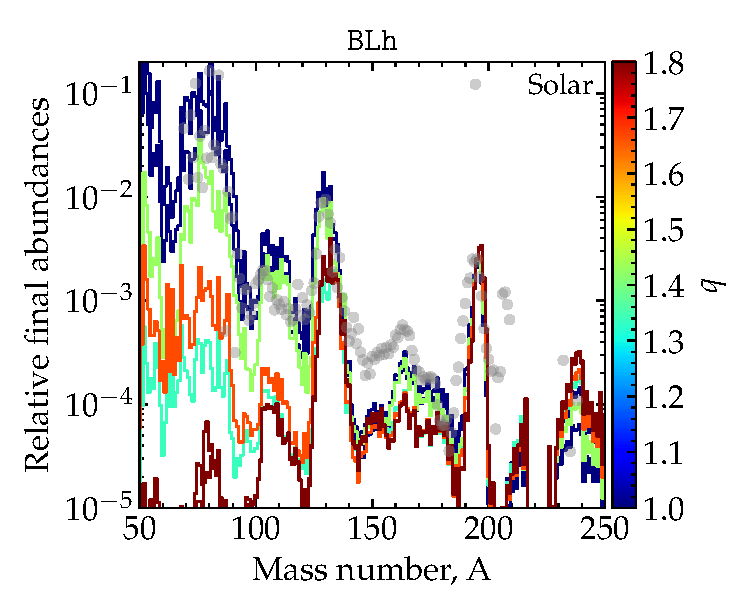
\includegraphics[width=0.45\textwidth]{nucleo/cc_nucleo_BLh_total.pdf}
    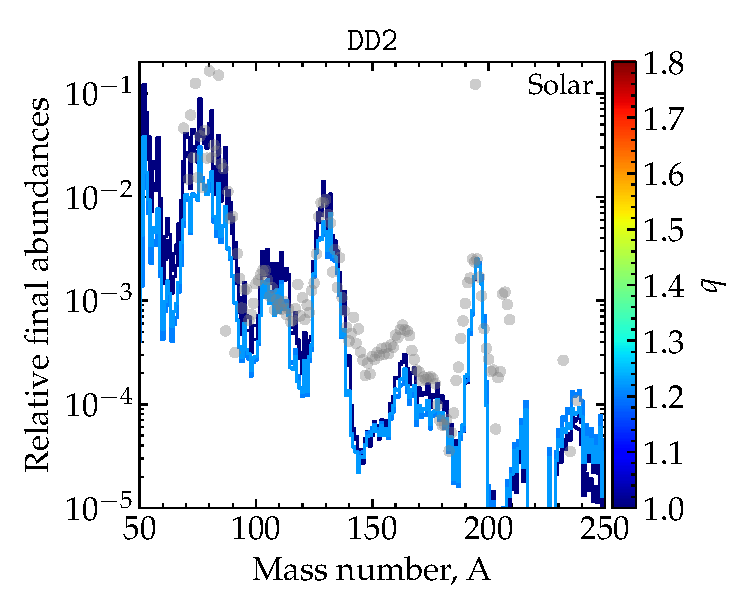
\includegraphics[width=0.45\textwidth]{nucleo/cc_nucleo_DD2_total.pdf}
    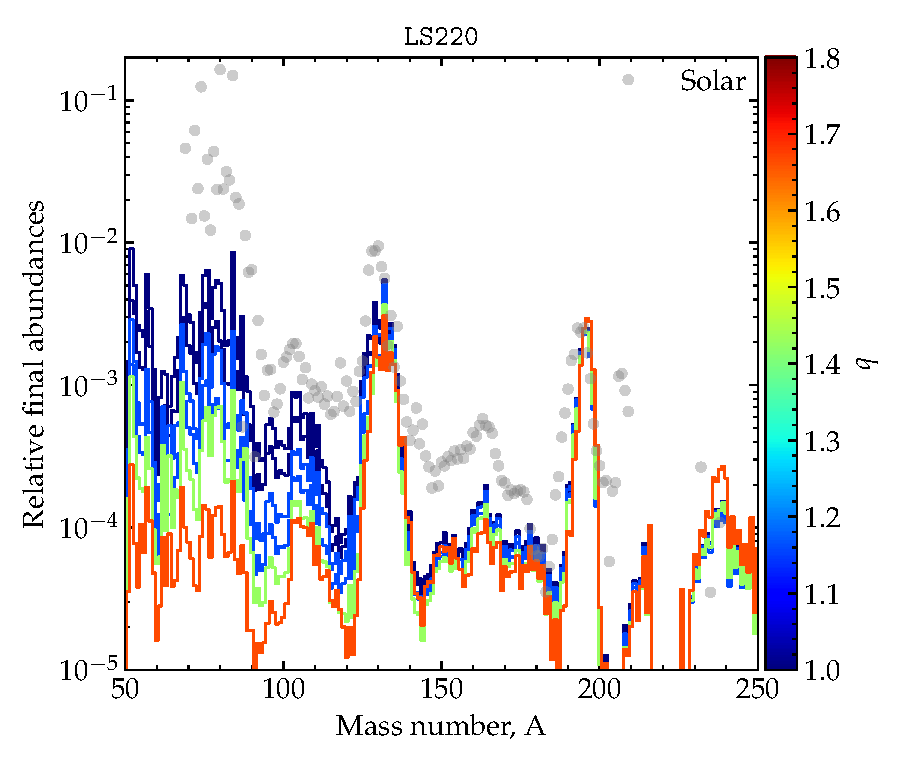
\includegraphics[width=0.45\textwidth]{nucleo/cc_nucleo_LS220_total.pdf}
    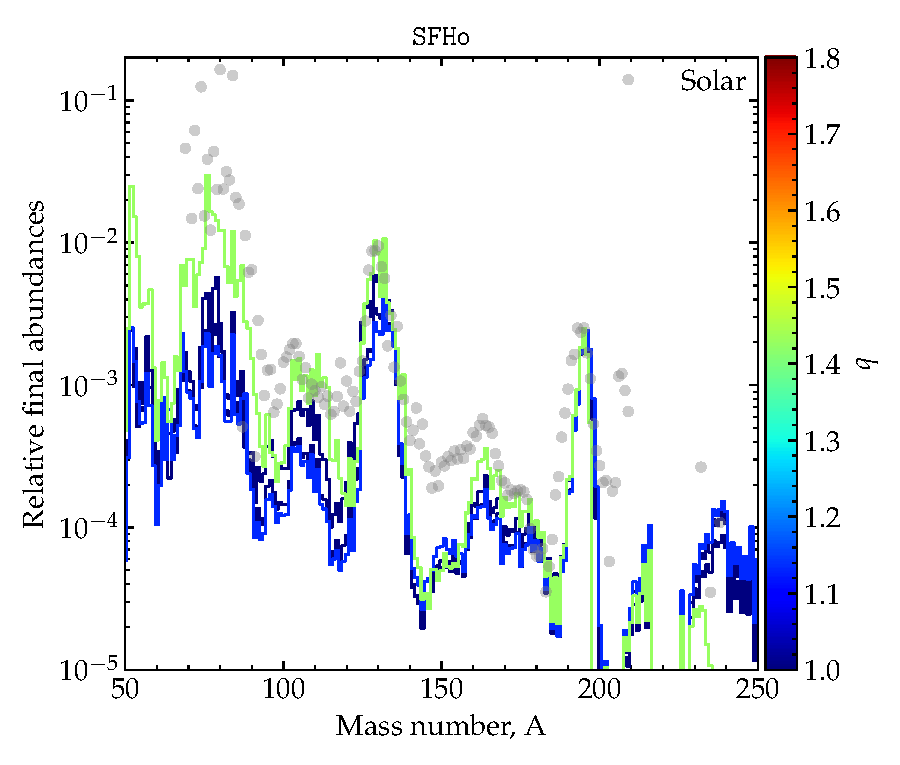
\includegraphics[width=0.45\textwidth]{nucleo/cc_nucleo_SFHo_total.pdf}
    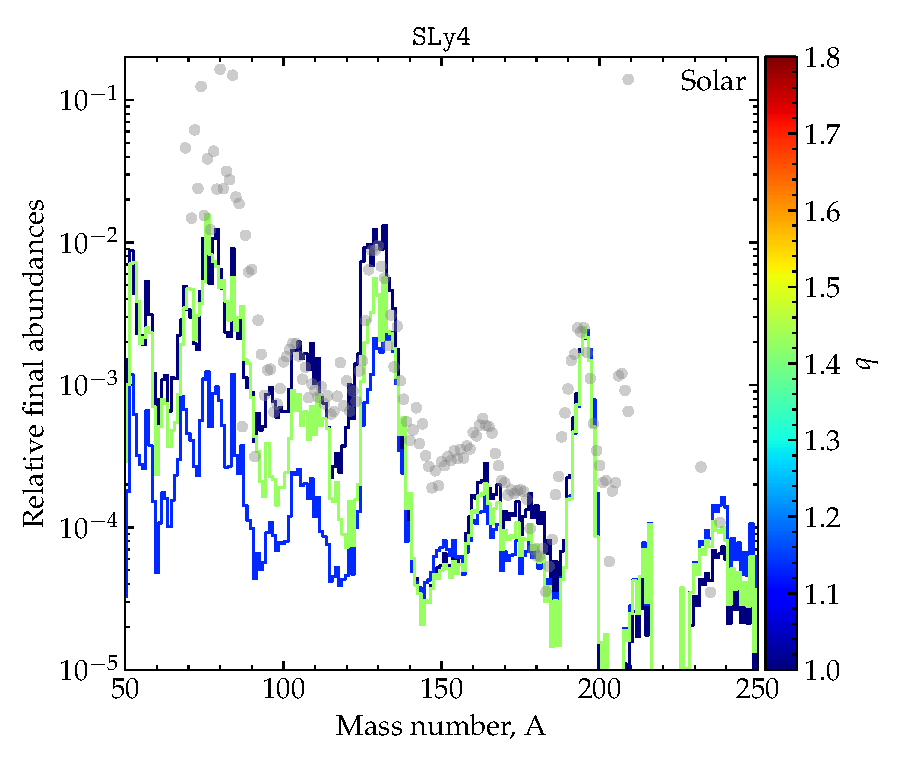
\includegraphics[width=0.45\textwidth]{nucleo/cc_nucleo_SLy4_total.pdf}
    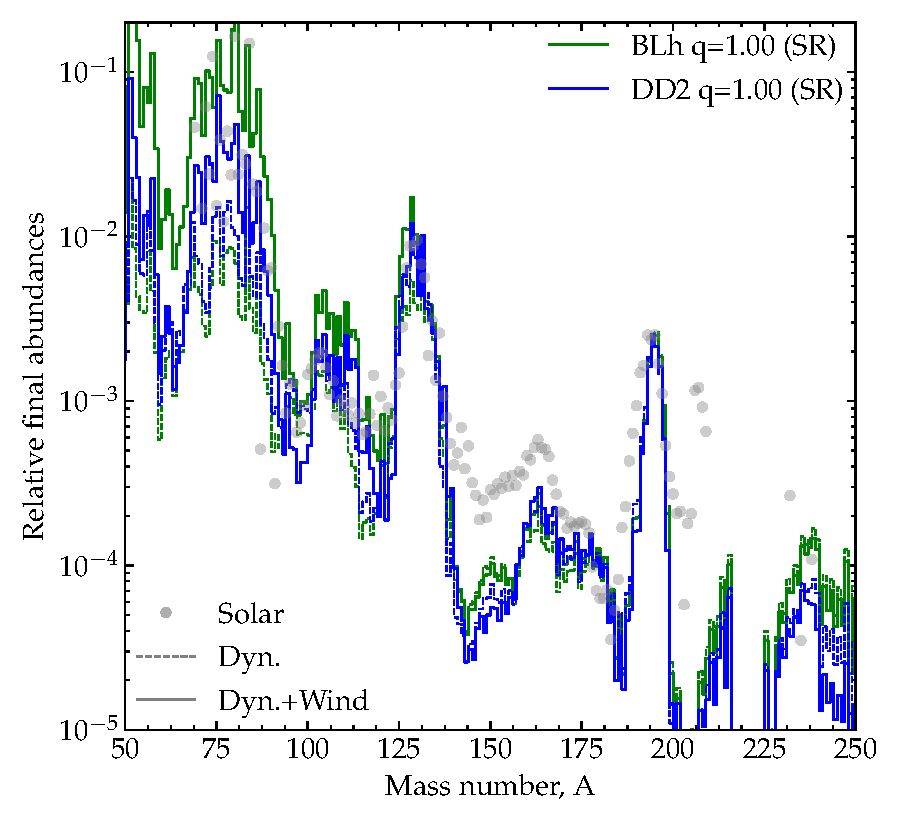
\includegraphics[width=0.42\textwidth]{nucleo/nucleo_dd2_blh.pdf}
    \caption{Nucleosynthesis yields for all simulations. Each %% panel
        of the first five panels 
        shows a different EOS and the scale color the dependency on the
        mass ratio. The nucleosynthesis is computed on the total ejecta
        computed during the simulations and 
        composed of the \ac{DE} (all models) plus the \ac{SWW} 
        (for the long-lived remnants listed in
        Tab.~\ref{tab:spiralwavewind}.).
        %
        The last (bottom-right) panel compares the nucleosynthesis in
        the \ac{DE} and \ac{SWW} for the long-lived
        remnants. The inclusion of the \ac{SWW} contributes to 
        improve the agreement with solar data for elements around the first peak.
        (Adapted from \citet{Nedora:2020pak})
    }
    \label{fig:nucle:totalyields}
\end{figure*}



%% -------------------------------------

%However, part of the uncertainty lies in the yet insufficient understanding of the nucleosynthetic yields from the neutron star mergers. Here we study the $r-$process
%abundances from the mergers, focusing on the effect of mass-ratio and equation of state. Complimentary to the previous study \cite{Radice:2018pdn}, we include the post-dynamical ejecta, \textit{e.g.,} \swind, where the lifetime of the remnant is sufficiently long. \\
%
%For the nucleosynthesis calculations we employ the same approach as in \cite{Radice:2016dwd} and \cite{Radice:2018pdn} which we outline briefly. Consider the outflowing material, crossing the coordiante sphere surface with $R\approx294$km that satisfies the criteria to be unbound, (geodesic for the dynamical ejecta and Bernoulli for the \swind) the following properties. WE extract its electron fraction n $Y_{e,R}$, specific entropy $s_R$, velocity $\upsilon_R$ and the rest-mass density $\rho_{0,R}$. In addition, we assume that the following expansion of the material is homologous, \textit{i.e.,}
%
%\begin{equation}
%\rho_{0}(t) = \rho_{0,R}\Big(\frac{\upsilon_R}{cR}t\Big)^{-3}.
%\label{eq:nucleo:rho_t}
%\end{equation}
%
%Then we match the density decrease with radius, with the $\rho$ behavior available in the parameterized $r$-process calculations of \cite{Lippuner:2015gwa}
%
%\begin{equation}
%\rho_{0}(t) = \rho_{0}(s, Y_e, T=6\text{GK})\Big(\frac{3\tau}{et}\Big)^3,
%\label{eq:nucleo:rho_t_lipp}
%\end{equation}
%
%where $\tau$ is the expansion timescale, and $e$ is the constant $e\approxeq 2.718$. Matching the equations \ref{eq:nucleo:rho_t} and \ref{eq:nucleo:rho_t_lipp} yields $\tau$ as
%
%\begin{equation}
%\tau_d = \frac{eR}{3\upsilon_R}\Bigg(\frac{\rho_R}{\rho_0}\Bigg)^{1/3}.
%\end{equation}
%
%Nucleosynthesis network calculations allow for a homologous expansion  to precompute the yields as a function of $\{\rho_{0,R},s_R,Y_{e,R},\tau_R\}$. Binning the corresponding ejecta parameter space, we can then use this precomputed data to gauge the nucleosynthetic yields in every bin of ejecta. Summing them, we obtain the total yield. For the discussion of the uncertainty of this method, see \cite{Radice:2018pdn}. \\
%
%It is also worth noting other approaches to nucleosynthesis computations in ejecta. In principle, the method should involve tracking numerous isotopic abundances of the material, that is moving along the fluid flow, undergoing fission, mixing and spallation, accounting for the EOS dependent feedback to the underlying flow. This however would require modifications to the composition equation and would make models computationally very expensive. A simplification to this approach would be to ignore the backreaction of nucleosynthesis to the flow dynamics, following the composition changes of Lagrangian traces advocated by it. It is believed that fission, while producing entropy that alters the burning in non-trivial way, amounts to only marginally changing the flow dynamics of lightly bound material \vn{it is however interesting to see how this would change the \swind mass}. Thus, the tracer approach is reasonable approximation, that is widely used. The technical difference with respect to the arropach employed in this work, is that the density history $\rho(t)$ is tracked in the ejecta instead of the assumption of homologous expansion. The entropy $s_0$ and electron fraction $Y_{e,0}$ are extracted at the time $t_0$ and then evolved using a self-heating nuclear reaction network \cite{Freiburghaus:1999}. \\
%
%The comparison between tracer method and homologous expansion one is performed in \cite{Radice:2018pdn}. It was concluded that within a factor of two, methods yield similar results. However, several caveats were pointed out with respect to the errors arising in ignoring the actual density history ($25\%$). On the other had it was stated that due to the approximation of Eualian flow with Lagrangian the error of $\sim 40\%$ can be expected. \\
%
%Here, employing the homologous expansions method. We report the relative abundances of different isotopes synthesized by the $r$-process \red{32} years \vn{not sure where this number is set up} after the merger in the material ejected from the system. In the \textit{short-lived} cases this encompasses only the dynamical ejecta, while in the \textit{long-lived} ones (see table \ref{tab:wind}) it includes the \swind. As the electron fraction is the most important quantity determining the outcome of the $r$-process \cite{Lippuner:2015gwa,Radice:2016dwd}, we report it for selected \textit{long-lived} models in figure \ref{fig:ejecta:bern:hist}. In the figure \ref{fig:nucleo:dynvswind} we compare how the inclusion of the \swind changes the abundances of two representative models and in the figures \ref{fig:nucleo:dynonly} and \ref{fig:nucleo:dynvswind} we show the total abundances of a large  subset of models, investigating the effect of mass ration and EOS (without and with the inclusion of \swind respectively). In all cases, we compare our abundances with the up-to-date solar ones from \cite{Prantzos2020} (for a review of the solar system abundances see \textit{e.g.,} \cite{Pritychenko:2019xvf}). The latter are normalized to the sum of all elements, while the model abundances are normalized to the solar at $A=195$. This is justified as long as ejecta contains very neutron rich material, as the nuclear fission cycling leads to a robust profile that follows the third $r$-process peak \cite{Lippuner:2015gwa}.\\
%
%The \cite{Radice:2018pdn} presents the systematics of the nucleosynthetic yields of a large subset of models, for which neutrino re-absorption has been neglected. Here we extent this by performing a similar analysis albeit with the subset of models that include the neutrino re-absorption. In addition, the subgrid turbulence is included in most of our models. However, its effect is much weaker then the one of the mass-ratio. Indeed, the figure \ref{fig:nucleo:dynonly} shows a model's ability to reproduce the solar $1$st and $2$nd r-process peaks, at $A\sim 100$ and $A\sim 125$ respectively strongly depended on the mass-ratio. Higher $q$ models, whose dynamical ejecta is mostly of tidal tail origin with very low electron fraction show severe underproduction of light $r$-process material, while $q=1$ DD2 and BLh models are able to reproduce both peaks reasonably well. This is the result of inclusion of neutrino reabsortion as it increases the $Y_e$ of the shocked component of the ejecta \cite{Radice:2018pdn}. Note, however, that in \cite{Papenfort:2018bjk} the effect of $q$ was not found. But similar to both studies, with respect to the equation of state, we do not observe consistent changes between still anf soft ones. This has also been the case in the aforementioned study.\\
%
%Important to note the actinides production, elements with atomic number $A\sim 230$. It was previously reported that in binary neutron star merger ejecta these materiel is overproduced (see \textit{e.g.,} \cite{Giuliani:2019oot}). However, we hint that this conclusion might partially be motivated by a choice of normalization. If we employ the physically motivated normalization to $A = 195$ of solar abundances, we observe that the actinides abundances are consistent with solar. We also note that there is dependency on the mass-ratio, motivated once again, by the ejecta composition. The very low $Y_e$ of highly assymetric models leads to significant boost in actinides production. This is the case for $q=1.8$ of BLh and $q=1.67$ of LS220. \\
%
%Indeed, to explain the $^{232}$Th solar abundances the average electron fraction in the ejecta should lower and any of our models except promptly collapsing ones can achieve. This underlines the importance of such mergers for $r$-process nucleosynthesis. We however emphases, that with adopted in this work normalisation, we do not observe overproduction of actinides, that was reported in \cite{Holmbeck:2019xnd}. \\
%
%+
%In the \textit{long-lived} case, the dynamical ejecta amounts to a small fraction of the total mass of material leaving the system. The second, more massive component, is the \swind. Its overall high electron fraction (see Fig. \ref{fig:ejecta:bern:hist}) implies that the weak $r$-process is dominant one here and light elements $A<195$ are primarily produced. In figure \ref{fig:nucleo:dynvswind} we compare the relative abundances from nucleosynthesis in dynamical ejecta only, with the total ones. Owing to the normalization to the $3$rd peak, it is reproduced in both cases, and the important difference lies in the $1$st and $2$nd peaks. In case of BLh we see that solar abundances of even very light elements $A\sim75$ are robustly reproduced. However there is an overproduction of $A\sim 110$ and $A\sim 130$ elements. The DD2 model, on the other hand, shows an overall lower total abundances. This is attributed to the slightly lower average electron fraction in DD2 (Fig. \ref{fig:ejecta:bern:hist}) while the ejecta masses are very similar (Fig.\ref{fig:mej:bern}). \\
%
%In the figure \ref{fig:nucle:totalyields} we investigate the total mass-ratio dependence of the total abundances. It is important to emphasis that in \textit{short-lived} cases this is the abundances of the dynamical ejecta only. Thus we limit this discussion to the DD2 and BLh models, most of which are sufficiently long with only extreme high $q$ BLh ones being an exception. Notably, the abundances strong $q$ dependence observed in dynamical ejecta, is not present for total ejecta, and all the $r$-process peaks are reasonably well reproduced by all the \textit{long-lived} models. This is not too surprising owing to the robust properties of the \swind, that change only marginally between different models. \\
%
%Overall, we find that dynamical ejecta of asymmetric models in general underproduces the $1$st and $2$nd r-process peaks due to its low average electron fraction. Equal mass DD2 and BLh models however are able to reproduce these peaks. Meanwhile, the total ejecta of DD2 and $q<1.7$ BLh models reproduces both, $1$st and $2$nd r-process peaks reasonably well irrespective of the mass-ratio, showing that the complete solar $r$-process abundances can be recovered if the remnant is \textit{long-lived}. This further supports the hypothesis, that binary netuton stars are the prime source of $r$-process material in the Universe.\\
%
%It is however, important to note that nucleosynthetic yields are subjected to the choice of nuclear input data. In particular, the choice of fission fragment distributions and neutron induced fission rates may have a large impact on abundances in the region of the $1$st and $2$nd peaks \cite{Eichler:2014kma}. The symmetric fission fragment distributions used in our calculations does most likely underproduce material in this region. In addition, as the neutrino-matter interaction rates roughly scale with the square of the incoming neutrino energy. Thus, the nucleosynthetic yields depend on the details of the neutrino radiation spectra \cite{Foucart:2016rxm}. The energy integrated scheme, employed in this work, does not allow us to take this effect into account (see, however, \cite{Radice:2018pdn} where different neutrino energy distributions were studied). It was recently pointed out that the neutrino resonant oscillations and fast flavor conversion might occur in NS merger remnants \cite{Zhu:2016mwa,Frensel:2016fge,Deaton:2018ser}. This might modify the nucleosynthesis of light $r$-process elements \cite{Wu:2016pnw}. Thus there is a need for more sophisticated simulations with spectral neutrino transport taking into account the neutrino oscillations. \\
%
%In addition to the dynamical ejecta and \swind, the $r$-process nucleosynthesis occurs in the secular ejecta. In particular in neutrino-driven winds, where neutrino irradiation of the expanding ejecta considerably increases the electron fraction. If the velocity of the ejecta sufficiently low, the material achieves $Y_e$ given by the weak equilibrium in optically thin conditions with neutrinos \cite{Qian:1996xt}. During the early post merger phase this $(Y_e)_{eq}\leq 0.45$ which allows for a weak $r$-process nucleosynthesis of light elements $A<130$ to occur \cite{Dessart:2008zd,Perego:2014fma,Foucart:2016rxm,Martin:2015hxa}. In addition, is expected that the dominant source of ejecta from the merger is the viscously-driven outflow from massive disk, if it forms after the merger. Properties on such outflow has been recently investigated in a framework of axisymmetric BH-torus systems \cite{Fernandez:2013tya,Just:2015fda}. The $Y_e$ distribution was found to be broad allowing all $r$-process elements from the $1$st to the $3$rd peak, as well actinides, to be synthesized in proportions close to solar (\textit{e.g.,} \cite{Wu:2016pnw}). If the \textit{long-lived} remnant is present however, the properties of the viscous ejecta are expected to be significantly altered by the large amount of neutrinos emitted over the diffusion time scale (seconds, \textit{e.g.,} \cite{Dessart:2008zd,Perego:2017fho}). 



%% -------------------------------------



%\red{Radice:2018pdn disussion on the accuracy}.

%\red{Something to check}
%\gray{
%    We do not nd material with expansion timescale of
%    less than 0.5 ms. This seems to exclude the neutron freezeout
%    scenario proposed by Metzger et al. (2015). However,
%    the lack of a very fast component of the ejecta might also
%    be due to numerical effects. Our resolution is probably not
%    high enough to track the very small fraction of the ejecta
%    expected to experience neutron freeze-out in the scenario
%    proposed by Metzger et al. (2015).
%}


%% ----------- results ----------------- 

With the procedure outlined above we compute the isotopic abundances of 
the \rproc{} elements $32$~years after merger. 
%% ---
The novelty of this analysis with respect to the previous study by 
\citep{Radice:2016dwd,Radice:2018pdn}, that used the same code and similar 
numerical setup, is that we have 
%
%Our analysis is the continuation of the previous study of the \ac{BNS} merger ejecta 
%\nuc{} conducted by \citet{Radice:2018pdn}. While we employ the same method
%to compute the abundances, the \ac{NR} simulations of our sample are 
(i) M0 neutrino scheme in all models, 
%
%In comparison with the previous study of the \ac{BNS} merger ejecta \nuc{} 
%conducted by \citet{Radice:2018pdn} with the same method, our \ac{NR} \ac{BNS} models include
%neutrino self absorption, 
(ii) and the effects of the subgrid turbulence in most models, 
(iii) which span a greater range in terms of \mr{} $q\geq1.8$,
and finally (iv) we consider several types of ejecta, \eg, \ac{DE}, \ac{SWW}.



In the Fig.~\ref{fig:nucle:totalyields} (except for the bottom right panel), 
we show the nucleosynthesis yields from overall ejecta.
% with each panel encompassing models with a given \ac{EOS} (the \mr{} is color-coded).
For models with short-lived \ac{MNS} remnants the total ejecta is comprised 
of the \ac{DE} only, while for models with long-lived ones, the total ejeta 
consists of \ac{DE} and \ac{SWW}. 
%
We compare the model abundances with the recently updated solar residual 
\rproc{} abundances from \citet{Prantzos2020},
%(and the recent overview on the topic can be found in \eg~\citet{Pritychenko:2019xvf})
%
multiplying the model abundances by a constant factor that brings the abundances 
at $A=195$ to that of the solar. This normalization allows to quantitatively 
assess relative abundances in different models.
%
%employing the following normalization.
%%For the qualitative comparison between models and observations we employ 
%%the following normalization. 
%The model abundances are multiples by a constant factor that makes the abundances at 
%$A=195$ equal solar.
%
From the plot we observe that the final \rproc{} abundances in the ejecta of models 
with moderately soft \acp{EOS} DD2 and BLh, that form long-lived remannts, are in 
good agreement with solar across all three \rproc{} peaks. .
%that 
%form long-lived \ac{NS} remnants with DD2 and BLh \acp{EOS}, are in agreement with 
%solar across all three \rproc{} peaks. 
This is because the \ac{DE} is a robust source of heavy elements with its low 
$Y_e$, that leads to fission cycling (see Sec.~\ref{sec:intro:nucleo}) and 
consistent reproduction of $2$nd and $3$rd \rproc{} elements; 
and \ac{SWW} being a robust source of lighter, $1$st and $2$nd peak elements
with its moderatly high electron fraction.
%This can be attributed to the combination of the low-$Y_e$ \ac{DE} -- the source of heavy 
%$2$nd and $3$rd \rproc{} elements are produced robustly due to fission cycling 
%(see Sec.~\ref{sec:intro:nucleo}), 
%and high-$Y_e$ \ac{SWW} with robust properties, where lighter elements, mostly at the 
%first peak are produced. 
%
With respect to the models with short-lived remnants, the final \rproc{} abundances 
at solar $1$st and $2$nd \rproc{} peaks, 
%(at $A\sim 75$ and $A\sim 125$ respectively) 
depend strongly on \mr{}. 
For instance, models with high $q$ have \ac{DE} of tidal origin mostly with low 
electron fraction. The final \rproc{} abundances in this ejecta show the underproduction 
of light elements. 
The final abundances in ejecta from equal mass binaries, 
however, display the presence of light \rproc{} elements which can be attributed 
tho the neutrino reabsorption raising the electron fraction 
in the shocked component of the \ac{DE} \citep{Wanajo:2014wha,Radice:2018pdn}. 

%% --- 
We observed that final abundances in the ejecta in all our models show the 
presence of actinides, elements with $A\sim230$. 
The amount of actinides produced, however, depends strongly on the ejecta 
electron fraction, and thus, on the binary \mr{}.
The agreement with solar abundances is found only for very asymmetric binaries. 
Notably, only for the binaries with the highest \mr{}, $q\sim1.8$, the 
\rproc{} in the \ac{DE} results in both $3$rd peak and actinides (at $^{232}$Th) abundances 
close to solar values. 
This suggests that the high \mr{} mergers or \ac{NSBH} mergers might be an 
important contributor to the cosmic chemical evolution.

%%--- Bottom right panel
The total ejecta from the models with long-lived \ac{NS} remnants is dominated by
the \ac{SWW}, as its mass is generally limited by the remnant lifetime 
(see Sec.~\ref{sec:bns_sims:ejecta}). 
In the bottom-right panel of Fig.~\ref{fig:nucle:totalyields} we show separately the 
final abundances from the \rproc{} in the \ac{DE} and in the \ac{DE} plus \ac{SWW}. 
The electron fraction of the \ac{SWW} is higher than that of the \ac{DE} 
%(see Fig.~\ref{fig:ejecta:bern:hist}), 
and thus the \rproc{} nucleosynthesis in the 
\ac{SWW} produces primarily light elements around the first \rproc{} peak, $A<95$\footnote{
    Note, that due to the choice of the normalization, all abundances are up-scaled 
    to reproduce the $A=195$ peak. Here the relative abundances at $1$st and $2$nd
    \rproc{} peaks are compared.
}.
%
The plot shows that for the models with BLh \ac{EOS} the amount of lighter elements, 
$A\sim75$, is higher with respect to the model with DD2 \ac{EOS}. This can be attributed 
to the higher electron fraction in the \ac{SWW} of the former (see Fig.~\ref{fig:ejecta:bern:hist}).
In both cases, however, the abundances of light elements are very close to solar. 
%\red{can be extended by adding plot from the Letter}


%% --- other ejecta types
The \rproc{} is expected to take place in other types of ejecta from \ac{BNS} mergers.
In \nwind{} the neutrino irradiation raises the electron fraction, which, depending 
on the ejecta velocity, can reach the $Y_e\leq 0.45$ \citep{Qian:1996xt}. 
At this pint the weak equilibrium sets in between the ejecta and neutrinos.
High electron fraction implies that only the light elements will be produced.
The numerical studies indeed support this picture 
\citep{Dessart:2008zd,Perego:2014fma,Just:2014fka,Martin:2015hxa,Foucart:2016rxm}. 

The bulk of the ejecta from \ac{BNS} mergers is expected to come in the form of 
viscous- and recombination-driven winds. This ejecta, however, is expected to take 
place over the longer timescales than those of our simulations.
Studies have shown that this ejecta has a broad distribution of the electron fraction.
The \rproc{} \nuc{} within it would produce light as well as heavy elements
\citep{Fernandez:2013tya,Just:2014fka,Wu:2016pnw,Siegel:2017nub,Fujibayashi:2017puw,Fernandez:2018kax}.
The production of the heavy \rproc{} elements, however, might be supressed in these winds
if the long-lived \ac{NS} is present \citep{Metzger:2014ila,Lippuner:2017bfm}.